\documentclass{beamer}
%\documentclass[handout]{beamer}
\usetheme{Darmstadt}

\usepackage[utf8]{inputenc}
\usepackage{default}
\usepackage{hyperref}

\newcommand{\tango}{\textsc{Tango}}
\newcommand{\corba}{\textsc{Corba}}
\newcommand{\onmiORB}{\textsc{omniORB}}
\newcommand{\zmq}{\textsc{$\varnothing$mq}}
\newcommand{\mysql}{\textsc{MySQL}}
\newcommand{\sardana}{\textsc{Sardana}}
\newcommand{\mambo}{\textsc{Mambo}}
\newcommand{\atk}{\textsc{Atk}}
\newcommand{\taurus}{\textsc{Taurus}}

\newcommand{\todo}[1]{\texttt{\color{red}TODO:} ``\emph{#1}''}

\title[Securing \tango\, Control System]{Securing \tango\, Control System:\\ A brain storming}
\author[Sergi Blanch-Torn\'e]{Sergi Blanch i Torn\'e}
\institute[Universidad de Lleida]{Cryptography \& Graphs\\Math Department\\ Universitat de Lleida}
\date{September 24th, 2013}

\begin{document}

%------------------------------------ Frame 0.1 ------------------------------%
%\frame{\titlepage}
\begin{frame}
  \titlepage
\end{frame}
%-----------------------------------------------------------------------------%

%------------------------------------ Frame 0.2 ------------------------------%
\begin{frame}
\frametitle{Outline}
\tableofcontents[hideallsubsections]
\end{frame}
%-----------------------------------------------------------------------------%

%%%%%%%%%%%%%%%%%%%%%%%%%%%%%%%%%%%%%%%%%%%%%%%%%%%%%%%%%%%%%%%%%%%%%%%%%%%%%%%
\section{Introduction}

\subsection{Definitions}

%------------------------------------ Frame 1.1 ------------------------------%
\begin{frame}
\frametitle{What is an Industrial Control System? (ICS)}
    \begin{block}{\href{http://en.wikipedia.org/wiki/Industrial_Control_System}{Wikipedia's definition (en)}}
        ``It is a general term that encompasses several types of control systems used in industrial production, including \emph{supervisory control and data acquisition} (SCADA) systems, \emph{distributed control systems} (DCS), and other smaller control system configurations such as \emph{programmable logic controllers} (PLC) often found in the industrial sectors and critical infrastructures.''
    \end{block}
    \begin{exampleblock}{Examples of an Industrial Control System}
        \todo{Add sample pictures here...}
    \end{exampleblock}
\end{frame}
%-----------------------------------------------------------------------------%

%------------------------------------ Frame 1.2 ------------------------------%
\begin{frame}
\frametitle{What is an SCADA?}
    \begin{block}{\href{http://es.wikipedia.org/wiki/SCADA}{Wikipedia's definition (es)}}
        ``\emph{Supervisory Control And Data Acquisition} it is a computer software to control and supervise industrial process remotely.''
    \end{block}
    \begin{exampleblock}{Examples of an SCADAs}
        \todo{Add sample pictures here...}
    \end{exampleblock}
\end{frame}
%-----------------------------------------------------------------------------%

%------------------------------------ Frame 1.3 ------------------------------%
\begin{frame}
\frametitle{What is an DCS?}
    \begin{block}{\href{http://en.wikipedia.org/wiki/Distributed_control_system}{Wikipedia's definition (en)}}
        a \emph{Distributed Control System} is the computer software for a manufacturing system, process or any kind of dynamic system, in which the controller elements are not central in location (like the brain) but are distributed throughout the system with each component sub-system controlled by one or more controllers.
    \end{block}
    \begin{block}{What is a distributed system?}
        Tanenbaum say \cite{TanenbaumDistr}: \emph{A distributed system is a collection of independent computers that appears to its users as a single coherent system.}
    \end{block}
\end{frame}
%-----------------------------------------------------------------------------%

%------------------------------------ Frame 1.4 ------------------------------%
\begin{frame}
\frametitle{What is a \tango? (I)}
    \begin{block}{The sea of Hardware}
        \todo{Add the nice picture of the shark...}
    \end{block}
\end{frame}
%-----------------------------------------------------------------------------%

%------------------------------------ Frame 1.5 ------------------------------%
\begin{frame}
\frametitle{What is a \tango? (II)}
    \begin{block}{It's an Distributed Control System}
          using \corba\, as a Middleware
    \end{block}
    \begin{block}{What means middleware?}
        Tanenbaum say \cite{TanenbaumDistr}: \emph{It is what supports heterogeneous computers and networks while offering a single system view.}
    \end{block}
\end{frame}
%-----------------------------------------------------------------------------%

%------------------------------------ Frame 1.6 ------------------------------%
\begin{frame}
\frametitle{What is a \tango? (iIII)}
    \begin{block}{\tango\, parts}
        \begin{itemize}
            \item \tango\, core $\Rightarrow$ the Middleware
            \item \tango\, Device Servers $\Rightarrow$ the agents in the DCS
        \end{itemize}
    \end{block}
    \begin{exampleblock}{Device servers, device classes, and devices}
        \todo{Draw a nice picture about what those three things are...}
    \end{exampleblock}
    \begin{block}{What has an Agent (a device)}
        \begin{itemize}
            \item Data types: Boolean, [U]Short, [U]Long[64], Double, String
            \item Data dimensions: Scalar, Spectrum, Image
        \end{itemize}
        \todo{commands,attributes and properties}
    \end{block}
% communications:
% - synchronous/asynchronous => \onmiORB
% - events => \zmq
% persistent data and phone book of the distributed system
% - tango-db => \mysql
% Framework:
% - \sardana
% Archiving:
% - Mambo
% User access:
% - \atk
% - \taurus
\end{frame}
%-----------------------------------------------------------------------------%

\subsection{Use cases of \tango}

%------------------------------------ Frame 1.7 ------------------------------%
\begin{frame}
\frametitle{Optics Lab: Long Term Profiler}
\end{frame}
%-----------------------------------------------------------------------------%

%------------------------------------ Frame 1.8 ------------------------------%
\begin{frame}
\frametitle{A beamline}
\end{frame}
%-----------------------------------------------------------------------------%

%------------------------------------ Frame 1.9 ------------------------------%
\begin{frame}
\frametitle{Control a synchrotron accelerator}
\end{frame}
%-----------------------------------------------------------------------------%

%%%%%%%%%%%%%%%%%%%%%%%%%%%%%%%%%%%%%%%%%%%%%%%%%%%%%%%%%%%%%%%%%%%%%%%%%%%%%%%
\section{Identify Scenarios}

\subsection{In distributed system}

%------------------------------------ Frame 2.1 ------------------------------%
\begin{frame}
\frametitle{Against the transparencies}
    \begin{tabular}{|l|l|}
        \hline
        Access & Hide differences in data representation and how a resource is accessed \\ \hline
        Location & Hide where a resource is located \\ \hline
        Migration & Hide that a resource may move to another location \\ \hline
        Relocation & Hide that a resource may be moved to another location while in use \\ \hline
        Replication & Hide that a resource is replicated \\ \hline
        Concurrency & Hide that a resource may be shared by several competitive users \\ \hline
        Failure & Hide a faulure and recovery of a resource \\ \hline
        Persistence & Hide whether a (software) resource is in memory or on disk \\ \hline
    \end{tabular}
\end{frame}
%-----------------------------------------------------------------------------%

%------------------------------------ Frame 2.2 ------------------------------%
\begin{frame}
\frametitle{Against the layers}
    \begin{figure}[h]
        \centering{
        %\resizebox{0.5\textwidth}{!}{% PSTricks TeX macro
% Title: /home/serguei/src/Papers/Ensuring_Tango_CtrlSys/imgs/TanenbaumDistributedSystemOrganization.dia
% Creator: Dia v0.97.2
% CreationDate: Sun Aug 11 19:16:03 2013
% For: serguei
% \usepackage{pstricks}
% The following commands are not supported in PSTricks at present
% We define them conditionally, so when they are implemented,
% this pstricks file will use them.
\ifx\setlinejoinmode\undefined
  \newcommand{\setlinejoinmode}[1]{}
\fi
\ifx\setlinecaps\undefined
  \newcommand{\setlinecaps}[1]{}
\fi
% This way define your own fonts mapping (for example with ifthen)
\ifx\setfont\undefined
  \newcommand{\setfont}[2]{}
\fi
\pspicture(3.900000,-19.100000)(24.100000,-5.386312)
\psscalebox{1.000000 -1.000000}{
\newrgbcolor{dialinecolor}{0.000000 0.000000 0.000000}%
\psset{linecolor=dialinecolor}
\newrgbcolor{diafillcolor}{1.000000 1.000000 1.000000}%
\psset{fillcolor=diafillcolor}
\psset{linewidth=0.100000cm}
\psset{linestyle=solid}
\psset{linestyle=solid}
\setlinejoinmode{0}
\newrgbcolor{dialinecolor}{0.000000 0.000000 0.000000}%
\psset{linecolor=dialinecolor}
\pspolygon(4.000000,7.000000)(4.000000,17.000000)(9.690000,17.000000)(9.690000,7.000000)
\psset{linewidth=0.100000cm}
\psset{linestyle=solid}
\psset{linestyle=solid}
\setlinejoinmode{0}
\newrgbcolor{dialinecolor}{0.000000 0.000000 0.000000}%
\psset{linecolor=dialinecolor}
\pspolygon(11.000000,7.000000)(11.000000,17.000000)(16.690000,17.000000)(16.690000,7.000000)
\psset{linewidth=0.100000cm}
\psset{linestyle=solid}
\psset{linestyle=solid}
\setlinejoinmode{0}
\newrgbcolor{dialinecolor}{0.000000 0.000000 0.000000}%
\psset{linecolor=dialinecolor}
\pspolygon(18.000000,7.000000)(18.000000,17.000000)(23.690000,17.000000)(23.690000,7.000000)
\psset{linewidth=0.100000cm}
\psset{linestyle=solid}
\psset{linestyle=solid}
\setlinejoinmode{0}
\newrgbcolor{dialinecolor}{1.000000 1.000000 1.000000}%
\psset{linecolor=dialinecolor}
\pspolygon*(5.000000,11.000000)(5.000000,13.000000)(23.000000,13.000000)(23.000000,11.000000)
\newrgbcolor{dialinecolor}{0.000000 0.000000 0.000000}%
\psset{linecolor=dialinecolor}
\pspolygon(5.000000,11.000000)(5.000000,13.000000)(23.000000,13.000000)(23.000000,11.000000)
\setfont{Helvetica}{0.800000}
\newrgbcolor{dialinecolor}{0.000000 0.000000 0.000000}%
\psset{linecolor=dialinecolor}
\rput(14.000000,12.000000){\psscalebox{1 -1}{Tango Middleware}}
\psset{linewidth=0.100000cm}
\psset{linestyle=solid}
\psset{linestyle=solid}
\setlinejoinmode{0}
\newrgbcolor{dialinecolor}{1.000000 1.000000 1.000000}%
\psset{linecolor=dialinecolor}
\pspolygon*(5.000000,8.000000)(5.000000,10.000000)(23.000000,10.000000)(23.000000,8.000000)
\newrgbcolor{dialinecolor}{0.000000 0.000000 0.000000}%
\psset{linecolor=dialinecolor}
\pspolygon(5.000000,8.000000)(5.000000,10.000000)(23.000000,10.000000)(23.000000,8.000000)
\setfont{Helvetica}{0.800000}
\newrgbcolor{dialinecolor}{0.000000 0.000000 0.000000}%
\psset{linecolor=dialinecolor}
\rput(14.000000,9.000000){\psscalebox{1 -1}{Distributed application}}
\psset{linewidth=0.100000cm}
\psset{linestyle=solid}
\psset{linestyle=solid}
\setlinejoinmode{0}
\newrgbcolor{dialinecolor}{0.000000 0.000000 0.000000}%
\psset{linecolor=dialinecolor}
\pspolygon(5.000000,14.000000)(5.000000,16.000000)(9.000000,16.000000)(9.000000,14.000000)
\setfont{Helvetica}{0.800000}
\newrgbcolor{dialinecolor}{0.000000 0.000000 0.000000}%
\psset{linecolor=dialinecolor}
\rput(7.000000,15.000000){\psscalebox{1 -1}{Local OS}}
\psset{linewidth=0.100000cm}
\psset{linestyle=solid}
\psset{linestyle=solid}
\setlinejoinmode{0}
\newrgbcolor{dialinecolor}{0.000000 0.000000 0.000000}%
\psset{linecolor=dialinecolor}
\pspolygon(12.000000,14.000000)(12.000000,16.000000)(16.000000,16.000000)(16.000000,14.000000)
\setfont{Helvetica}{0.800000}
\newrgbcolor{dialinecolor}{0.000000 0.000000 0.000000}%
\psset{linecolor=dialinecolor}
\rput(14.000000,15.000000){\psscalebox{1 -1}{Local OS}}
\psset{linewidth=0.100000cm}
\psset{linestyle=solid}
\psset{linestyle=solid}
\setlinejoinmode{0}
\newrgbcolor{dialinecolor}{0.000000 0.000000 0.000000}%
\psset{linecolor=dialinecolor}
\pspolygon(19.000000,14.000000)(19.000000,16.000000)(23.000000,16.000000)(23.000000,14.000000)
\setfont{Helvetica}{0.800000}
\newrgbcolor{dialinecolor}{0.000000 0.000000 0.000000}%
\psset{linecolor=dialinecolor}
\rput(21.000000,15.000000){\psscalebox{1 -1}{Local OS}}
\psset{linewidth=0.200000cm}
\psset{linestyle=solid}
\psset{linestyle=solid}
\setlinecaps{0}
\newrgbcolor{dialinecolor}{0.000000 0.000000 0.000000}%
\psset{linecolor=dialinecolor}
\psline(4.000000,19.000000)(24.000000,19.000000)
\psset{linewidth=0.200000cm}
\psset{linestyle=solid}
\psset{linestyle=solid}
\setlinecaps{0}
\newrgbcolor{dialinecolor}{0.000000 0.000000 0.000000}%
\psset{linecolor=dialinecolor}
\psline(7.000000,17.000000)(7.000000,19.000000)
\psset{linewidth=0.200000cm}
\psset{linestyle=solid}
\psset{linestyle=solid}
\setlinecaps{0}
\newrgbcolor{dialinecolor}{0.000000 0.000000 0.000000}%
\psset{linecolor=dialinecolor}
\psline(14.000000,17.000000)(14.000000,19.000000)
\psset{linewidth=0.200000cm}
\psset{linestyle=solid}
\psset{linestyle=solid}
\setlinecaps{0}
\newrgbcolor{dialinecolor}{0.000000 0.000000 0.000000}%
\psset{linecolor=dialinecolor}
\psline(21.000000,17.000000)(21.000000,19.000000)
\setfont{Helvetica}{0.800000}
\newrgbcolor{dialinecolor}{0.000000 0.000000 0.000000}%
\psset{linecolor=dialinecolor}
\rput[l](5.000000,4.000000){\psscalebox{1 -1}{}}
\setfont{Helvetica}{0.800000}
\newrgbcolor{dialinecolor}{0.000000 0.000000 0.000000}%
\psset{linecolor=dialinecolor}
\rput(7.000000,6.000000){\psscalebox{1 -1}{Machine A}}
\setfont{Helvetica}{0.800000}
\newrgbcolor{dialinecolor}{0.000000 0.000000 0.000000}%
\psset{linecolor=dialinecolor}
\rput(7.000000,6.800000){\psscalebox{1 -1}{}}
\setfont{Helvetica}{0.800000}
\newrgbcolor{dialinecolor}{0.000000 0.000000 0.000000}%
\psset{linecolor=dialinecolor}
\rput(14.000000,6.000000){\psscalebox{1 -1}{Machine B}}
\setfont{Helvetica}{0.800000}
\newrgbcolor{dialinecolor}{0.000000 0.000000 0.000000}%
\psset{linecolor=dialinecolor}
\rput(21.000000,6.000000){\psscalebox{1 -1}{Machine C}
\endpspicture}
        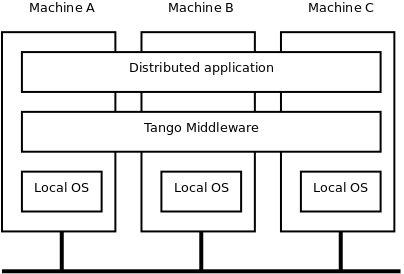
\includegraphics[width=0.5\textwidth]{imgs/TanenbaumDistributedSystemOrganization.png}
        \caption{From \cite{TanenbaumDistr}, A distributed system organized as middleware} \label{fig:TanenbaumDistributedSystemOrganization}}
    \end{figure}
\end{frame}
%-----------------------------------------------------------------------------%

\subsection{In security Engineering}

%------------------------------------ Frame 2.3 ------------------------------%
\begin{frame}
\frametitle{Basics}
    \begin{itemize}
        \item Confidentiality
        \item Authenticity
        \item Integrity
        \item Availability
        \item Non-repudiation
    \end{itemize}
\end{frame}
%-----------------------------------------------------------------------------%

%%%%%%%%%%%%%%%%%%%%%%%%%%%%%%%%%%%%%%%%%%%%%%%%%%%%%%%%%%%%%%%%%%%%%%%%%%%%%%%
\section{Security levels}

\subsection{Security threads}

%------------------------------------ Frame 3.1 ------------------------------%
\begin{frame}
\frametitle{Security levels}
    
\end{frame}
%-----------------------------------------------------------------------------%

\subsection{Labelling}

%------------------------------------ Frame 3.2 ------------------------------%
\begin{frame}
\frametitle{Security levels}
    European commission \emph{fiche 17} \\``Exchange of EU classified information'' \cite{fiche17EU}
    \begin{itemize}
        \item Open or Unclassified
        \item Confidential
        \item Secret
        \item Top-Secret
    \end{itemize}

\end{frame}
%-----------------------------------------------------------------------------%

%%%%%%%%%%%%%%%%%%%%%%%%%%%%%%%%%%%%%%%%%%%%%%%%%%%%%%%%%%%%%%%%%%%%%%%%%%%%%%%
\section{Proposed solutions}

% authentication of agents and users
% encryption of data transmitted:
% - solutions for synchronous/asynchronous
% - solutions for events
% secure the tango-db access: query and write

\subsection{Authentication}

%------------------------------------ Frame 4.1 ------------------------------%
\begin{frame}
\frametitle{Authentication}
\end{frame}
%-----------------------------------------------------------------------------%

\subsection{Encryption}

%------------------------------------ Frame 4.2 ------------------------------%
\begin{frame}
\frametitle{Encryption}
\end{frame}
%-----------------------------------------------------------------------------%

\subsection{Database}

%------------------------------------ Frame 4.3 ------------------------------%
\begin{frame}
\frametitle{Database access}
\end{frame}
%-----------------------------------------------------------------------------%

%%%%%%%%%%%%%%%%%%%%%%%%%%%%%%%%%%%%%%%%%%%%%%%%%%%%%%%%%%%%%%%%%%%%%%%%%%%%%%%
\section{Reference Papers}

%iacr
%arxiv
%scholar
%dblp

%------------------------------------ Frame 5.1 ------------------------------%
\begin{frame}
\frametitle{Reference Papers}
\end{frame}
%-----------------------------------------------------------------------------%

%%%%%%%%%%%%%%%%%%%%%%%%%%%%%%%%%%%%%%%%%%%%%%%%%%%%%%%%%%%%%%%%%%%%%%%%%%%%%%%
\section{Reference journals and conferences}

%------------------------------------ Frame 6.1 ------------------------------%
\begin{frame}
\frametitle{Reference journals and conferences}
\end{frame}
%-----------------------------------------------------------------------------%

%%%%%%%%%%%%%%%%%%%%%%%%%%%%%%%%%%%%%%%%%%%%%%%%%%%%%%%%%%%%%%%%%%%%%%%%%%%%%%%
\begin{frame}[allowframebreaks]
        \frametitle{References}
        %\bibliographystyle{amsalpha}
        \bibliographystyle{ieeetr}
        \bibliography{../bibtex/books.bib,../bibtex/standards.bib,}
\end{frame}


\end{document}


